\section{Teilaufgabe}

\subsection{k-Means Map und Reduce Pseudocode}
K-Means ist einer der bekanntesten Algorithmen zur Clusteranalyse. Dabei werden ähnliche Objekte zu einer Gruppe zusammengefasst. Die Ähnlichkeit wird durch den Abstand im Raum (Distanz) repräsentiert. 

Zu Beginn erwartet k-Means die Anzahl \emph{k} der gewünschten Cluster und erstellt daraufhin \emph{k} initiale Clusterzentren auf dem übergebenen Datensatz.

\begin{figure}[htb]
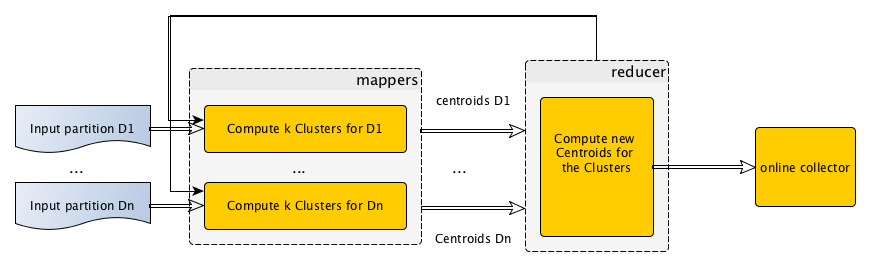
\includegraphics[scale=0.5]{MapReduceBild.png}
\centering
\caption{Überblick über die MapReduce Ausführug von k-Means}
\label{fig:MapRed}
\end{figure}

\subsubsection{Map}
Im Map-Schritt werden die Datenpunkte (WordVektoren) den Clustern zugewiesen. Als Output werden Key-Value-Paare mit dem Cluster als Key erwartet. 
\begin{lstlisting}[caption=Map Pseudocode,label=lst:map,numbers=left,xleftmargin=2em,
framexleftmargin=2em,morekeywords={FOREACH, IF, NULL}]

// Gegeben: Liste mit k initialen Clusterzentren, unsere Word-Vektoren
// Mit der Map-Funktion werden die Clusterzentren und ein Teil der Word-Vektoren als Argumente übergeben

Map (List<ClusterCenter> centers, List<WordVector> words) 

  FOREACH wordVector in words {
  
    minDistance = Double.MaxValue;
    nearestClusterCenter = NULL;  
  
    FOREACH center in centers {
      //Distanzmessung wie in Userdefined Function Cosinus-Ähnlichkeit 
      distance = measureDistance(center, word);
      IF(distance < minDistance) {
        minDistance = distance;
        nearestClusterCenter = center;
      }
    }
    
    //Speichere KeyValue Pair also WordVector zu dem Clusterzentrum 
    context.write(nearestClusterCenter, wordVector);
  }
}
\end{lstlisting}

\subsubsection{Reduce}

Im Reduce-Schritt werden für die Datenpunkte (WordVektoren) die Clustermittelpunkte berechnet und gespeichert. Der Input für den Reducer ist der sortierte Output des Mappers, also die Clusterzuordnungen. .
\begin{lstlisting}[caption=Reduce Pseudocode,label=lst:reduce,numbers=left,xleftmargin=2em,framexleftmargin=2em]
public void reducer(ClusterCenter key, Iterable<WordVector> values, Context context)
{
 //Summiere alle Vektoren auf
 vectorSum = null;
 FOREACH WordVektor in Wordvectors{
   VectorSum += Wordvector; 
 }
 
 CenterVector = VectorSum/VectorCount;
 CenterId = ClusterCenter.id;
 //Speichere KeyValue Pair also CenterId und Vector
 context.write(CenterId, CenterVector)
 //Zähler für Endbedingung
 context.UpdateCount;
 
}
\end{lstlisting}

\subsection{Initialisierung der Algorithmen}
Zu Beginn der Ausführung müssen die Clusterzentren initialisiert werden. Dabei wird für die gewünschte Anzahl an Clustern jeweils ein zufälliger Punkt als Clusterzentrum gewählt. Dafür muss der Seed in der Initialisierung gesetzt werden. Im laufe der Iterationen verscheiben sich diese dann immer stärker zu den eigentlichen Clusterzentren.

\subsection{Klassen und Methoden}
Für die Implementierung von Map-Reduce-Anwendungen werden einige User-Interfaces bereitgestellt. Anwendungen wie z.B. WordCount implementieren typischerweise die \textit{Map-} und \textit{Reduce-Klassen}. Die Map und die Reduce-Klasse werden in der Main-Methode über \textit{Job.setMapper(class)} bzw. \textit{Job.setReducer(class)}  gesetzt. Dies ist auch für den K-Means Algorithmus notwendig.

Für jeden InputSplit im InportFormat wird ein Job gestartet.

Die \textit{Mapper Klasse} soll neben der Map Schritt auch weitere Methoden zu implementieren. In der \textit{Setup-Methode} werden die notwendigen Initialisierungen vorgenommen und die Konfiguration durchgeführt. Auch eine Parse-Methode wird zum analysieren des Inputs benötigt. Für die Berechnung der Distanz im Map-Schritt ist eine Distanzmesser zu implementieren.

Die \textit{Reducer-Klasse} enthält die \textit{Reduce-Methode} welche die Clustermittelpunkte bilden soll.

Außerdem ist es für den Anwendungsfall sinnvoll ein Modell zu implementieren. Dies ist im WordCount-Beispiel nicht zu finden, was der Einfachheit des Beispiels geschuldet ist. Dies wird in der Main-Methode 			\textit{job.setOutputKeyClass(class)} und \textit{job.setOutputValueClass(class)} gesetzt. Sinvolle Klassen wären ClusterCenter und WordVector.
